\Chapter{The Business as I remember it}{Glyn Court}

The most subtle anatomist in the kingdom would be hard put to it to find any quantity of blue blood in my veins, and I summise that the somewhat sluggish liquid is rather a compound of red and white corpuscles, shoemaker's dye, machine oil and Post Office ink. At least, if one or the other of the last three is not traceable, then all talk of \quotemark{environmental conditioning} is mere psychiatrese.

The village post office of Washford, in which I grew up, was very exceptional. There is a strange fascination in the thought of one particular human activity being carried on in one unchanging spot as the generations come and go, and a few years ago I was enthralled to learn from a North Devon schoolboy that his family had been occupying their farm, of their own name, ever since the fifteenth century. The post office at Washford could not claim such a history, but for at least a century and a quarter, and probably for two centuries, the postal business of the community was carried on in two houses which faced each other across the village street - our house and the old office.

When my mother became the postmistress in 1921 and moved from the old place to her new home, no one knew how long the service had been operating: apparently it was for longer than that term within which, in the legal phrase, the memory of man runneth not to the contrary. Fifty years later this was confirmed to us, and in a surprising way, for our neighbour, who had bought the old post office cottage on the death of the former postmaster's daughter, set about remodelling the interior. He removed the entrance lobby which had been the telegraph room, and demolished a partition, and in behind this he found papers which had lain undisturbed for nearly 120 years: light green registered letter forms dated 1853 and showing - which tickled our vanity - Washford as the head office and Minehead as the humble sub-office. Even more surprising, another neighbour brought us in a brass button from the garden which, from its condition, had evidently lain in the earth for many, many years. It showed a head of an eighteenth-century type - we were tempted to assign it to George I since it faced to the right - and the letters P.D, which we took as indicating \quotemark{Postal Department}. The British Museum could not enlighten us as to the origin, so \quotemark{Postal Department} it remains, and we are convinced that this activity, in one way or another, has gone on here for at least two centuries.

Nevertheless, the business activity as a whole was much more varied. As my wife has explained, when my father was building the house, he added a single storey wing in sandstone and snail-creep to carry on the cycle and footwear trade; then, having an eye for symmetry, he continued the outside wall - only in brick and rough-cast, because of the expense - to make a second storey and roofed over the whole area. All the woodwork in the house came from his plane, and all the fittings in the shop were his work, too - not that any village store, in those innocent days, would have been fitted up by an outside agency: such a fall from grace was mercifully hidden in the future.

The post office and shop as I remember them from my boyhood were pretty constantly busy, as we catered for at least three sets of customers. In the 1920 we were still in the throes of the first Vehicular Revolution, and working men were buying Hercules and Raleigh cycles as eagerly as their sons and grandsons buy Rover 3000s, only less frequently and, comparatively speaking, at much greater cost. The second strand of the business was footwear, which my father had chosen to carry on because, as he shrewdly observed, \quotemark{Most of ’em have two feet, and they always need two shoes to put on 'em}. And both the cycle trade and the footwear gave rise to a moderately profitable repair business.

The third estate of our commercial empire was, of course, the post office. My mother had worked as an assistant for fifteen years in the post office over the way, and after her marriage she became the postmistress of Washford in her new home; and she held the position until the day of her death, forty-five years later.

Our shop was one huge room occupying the whole of the extension, but divided by a partition, with a floor laid in wooden blocks in herringbone pattern, and a ceiling of grooved and tongued deal. The shop front was mainly taken up by two huge plate-glass -windows set in frames part oak, part pine, and four inches thick, and the front door and porch were set in one corner.

The display window was generally occupied by one or two bicycles suspended from hooks, and a varied selection of shoes, slippers and cycle accessories. Along the right hand side of the shop ran the post office counter, a massive structure of red mahogany twelve feet long, purchased from the mess deck of a destroyer that was being broken up in Watchet harbour. The counter was surmounted by a brass grill and a kind of miniature signal-box or glass cabinet in which we kept a variety of official forms whose age-long incapacity for use rendered them inestimably precious in the sight of the Postmaster General. Underneath were five huge drawers, which might have served as coal barges but that they were crammed with post office supplies and forms; and underneath these were more shelves, all laden with post office envelopes in their scores, forms in their hundreds, and governmental trivia in their thousands and tens of thousands. At the far end of the counter stood the post office scales, solid, black, imposing, with a range of weights from an ounce to seven pounds; and there they stood until the late 1930s when the Post Office, recognising their dependability as unsuitable for a go-ahead public corporation, removed them.

Down the left side of the shop ran another stand of shelves on which were displayed electric lamps, greetings cards, flower and vegetable seeds, cycle parts, inner tubes and a selection of small goods of many and varying kinds. Behind this, and facing the door, was the telephone kiosk painted in a brown which seemed to have been evolved in the more secluded recesses of Bournville; through this kiosk we sent and received telegrams, sometimes ten or twelve a day. The telephone had the property of picking up the broadcasts from the local B.B.C. station, and I remember that, before we owned a wireless set, we heard over this improvised radio the abdication speech of King Edward VIII.

On one of the lower shelves was a commodity which was much prized up to the war but has now disappeared from daily use: calcium carbide, which we kept in cylindrical one pound tins and sold for fourpence. Well into the 1940s carbide cycle lamps were very popular in our area; for the carbide gave a brighter, clearer light than electric batteries. The men who cycled to and from the paper mill in Watchet would call in regularly between half-past five and six to exchange their empty carbide tin for a new one.

And along all three walls of the shop, piled up from waist level to ceiling, was the principal stock-in-trade, footwear: light boots, heavy boots, ladies' boots from before the Great War, Wellington boots, boots adorned with brads, tips and cues, hobnail boots in every size from the twelves for a six-foot farmer down to the tiny hobnail fours for a two year old toddler - or maybe hobbler; shoes of every probable shape, and not a few rankly improbable; \quotemark{I can always fit their feet}, said Father, who had no great love for the vagaries of female fashion; \quotemark{I can fit their feet, but I can't fit their heads.}: slippers and plimsolls, bootlaces and insoles (\quotemark{socks} they were called); and those perfect accoutrements for the ploughman behind his team, leathern leggings.

\begin{figure}
	\centering
     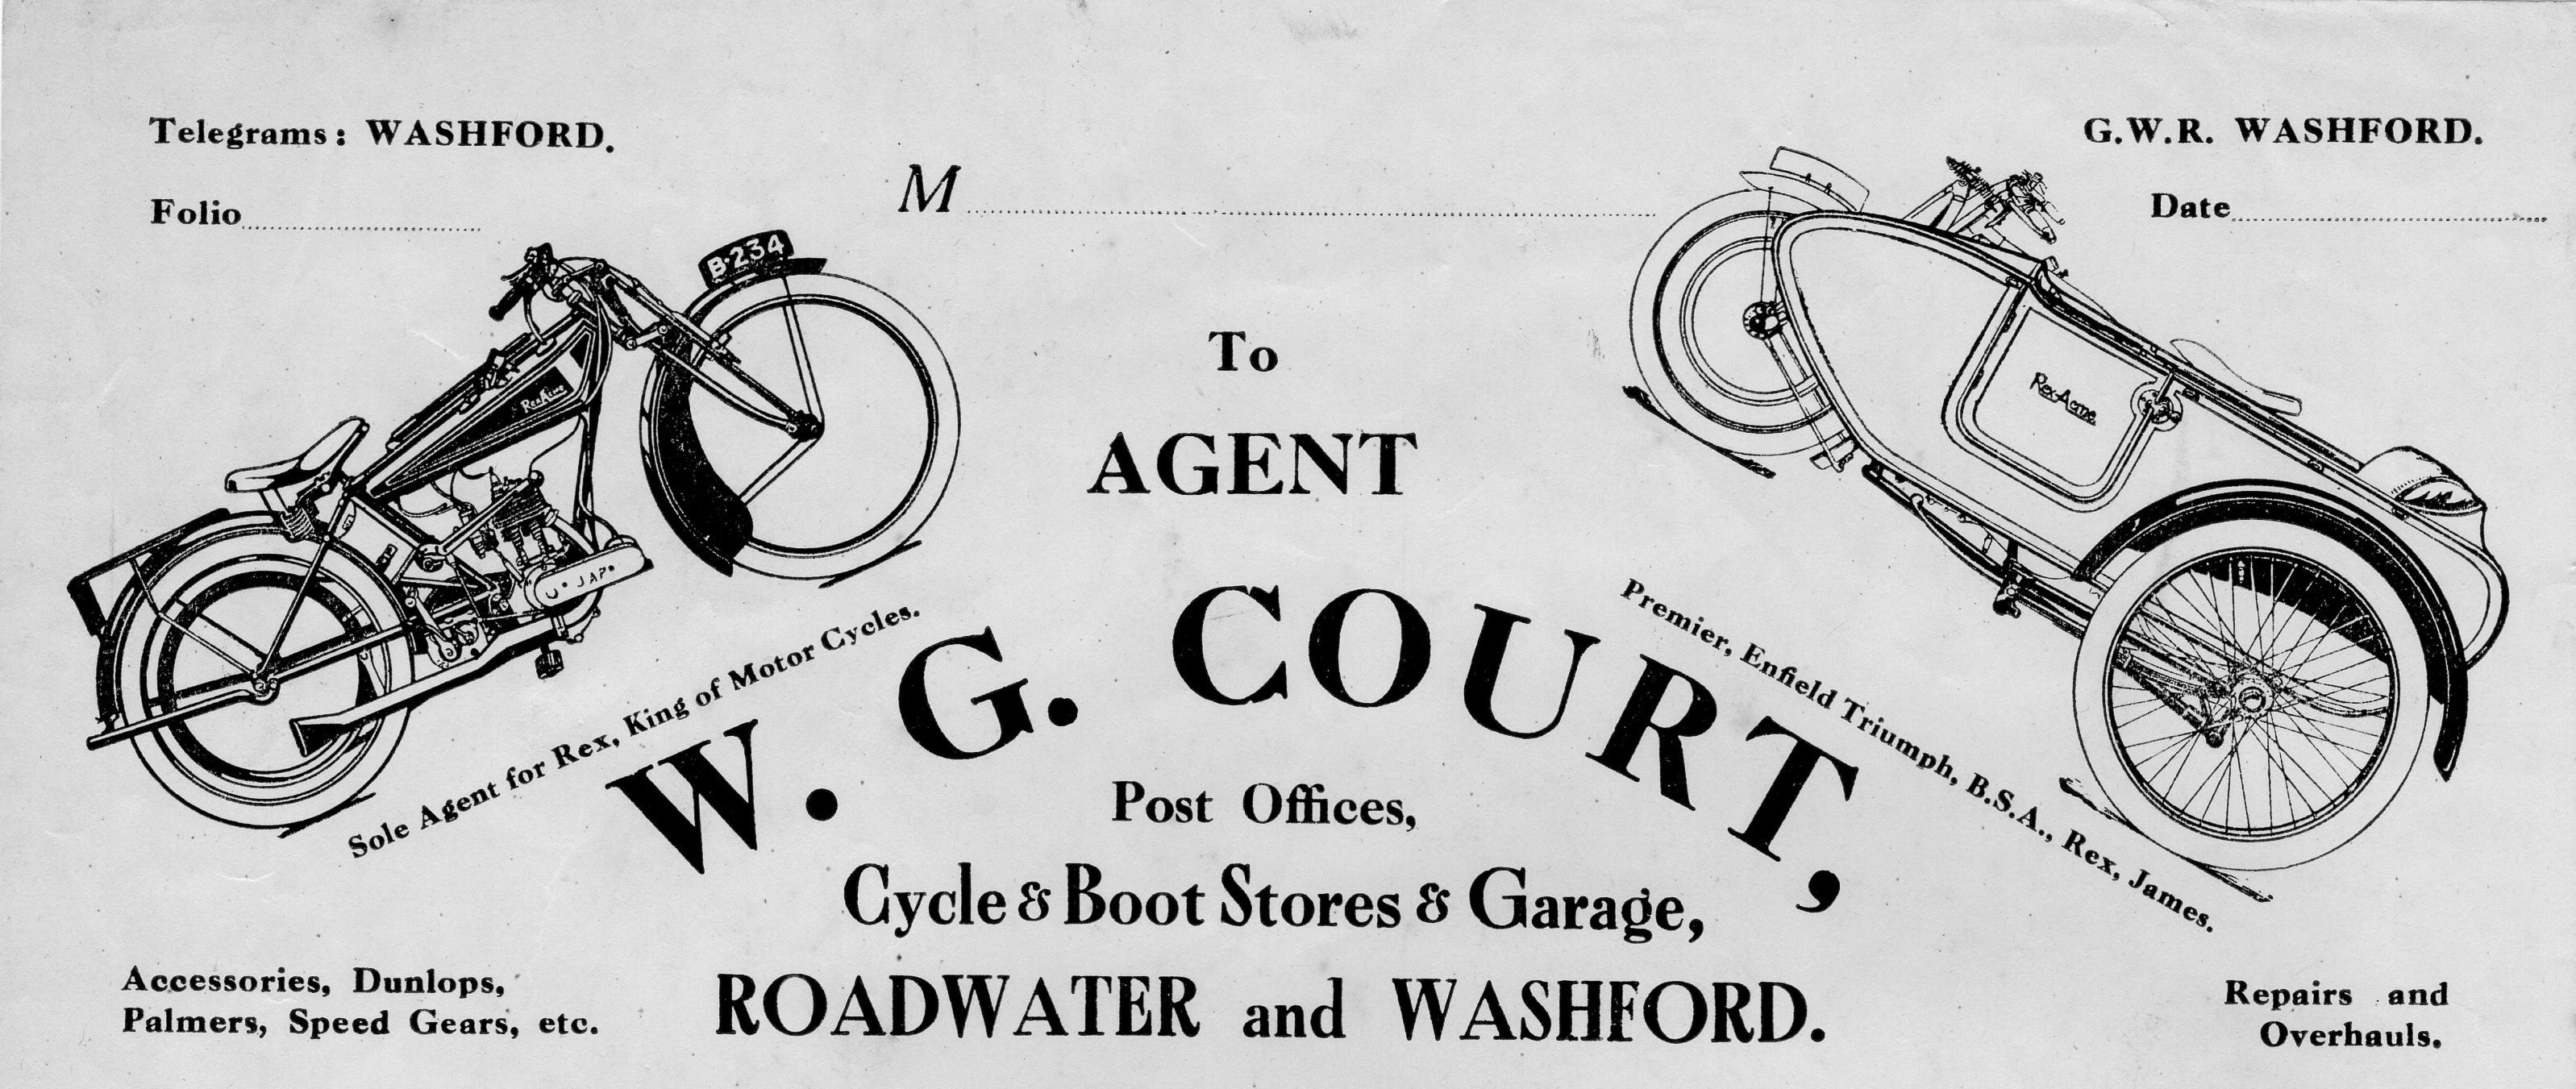
\includegraphics[width=1\textwidth]{figures/Receipt}
     \caption{The receipt header for the shop, highlighting the diverse range of services available at the post office.}
     \label{fig:Receipt}
\end{figure}

All these treasures were found in the front shop. Beyond the partition, and reached through a green baize curtain, lay the sorting office; on one side a boxed staircase led to the first floor. Along two of the other walls were the rows of shelves for the sorting of the letters and a desk for Father's business papers; and on the third side stood the telephone exchange, a standard which, for many years, had barely fifty numbers on it; but those fifty were sufficient to bind my mother and father to the service of the Post Office day and night for nearly twenty years.

The sorting office was busy out of all proportion to the usual work of a village post office, for by some quirk of authority we had been chosen as the centre of distribution for a large area - of West Somerset. Out two motor vans, one a bull-nosed Morris Cowley, the other an Oxford, covered the Brendon Hills and the eastern half of Exmoor, delivering mail to the scattered villages of Dunster, Wheddon Cross, Exford, Withypool, Winsford and a score of isolated farms. Another postman delivered the village and two girls served behind the counter.

Competition for employment as a postman was strong in the 1930s, and entry was practically restricted to ex-servicemen, so there was a peculiar fitness in the names of one of our postmen, Jim Lee, Bill Bellamy and Tommy Atkins. For those who were sociably inclined, the work was interesting; they met dozens of people on their rounds, and never exactly the same people two days running.

Sometimes, in the holidays, I would be allowed to travel in the mail van, and I have often suspected that those journeys did more than any other single experience to create in me the romantic frame of mind under which I have always laboured and for which, paradoxically, I am profoundly thankful. In winter we would set out from the office in darkness and pass through Dunster and Timberscombe as the lights still glowed in the cottage windows. As we climbed the thousand feet up to the Rest and Be Thankful at Wheddon Cross, the stars were paling and the beech hedges and the cairn of Dunkery were struggling out of darkness into the grey of morning. Then we would pay our visits to those villages of which I had so often heard but which, without the mail van, might have been at the ends of the earth, so little did children such as I travel outside their immediate neighbourhood: Exford, Winsford, Withypool, Luckwell Bridge. On other mornings I would travel with the Brendon Hill van and we would follow up the stream which came rushing from the windy uplands of Chargot and Leigh. For the first two miles, to Roadwater, I knew the country well, for the village held the home of my family; but beyond Roadwater, all was unknown, and as the road wound through the sombre pine-woods, and emerged into the higher pastures beside the stream, each new name had for me a quality of magic: Pittiwells Lake, Langridge Mills, Drucombe, New Mills, Greenland, Kingsbridge, Luxborough, Chargot. The hills drew me to themselves. We laboured up the steep of Vellers Way or, I had been told, Felon's Way, and I vaguely wondered who had been the malefactor and what his crime. Sheep stealing, maybe?

Twelve hundred feet above sea level now, and we visited one remote farmstead after another: Burrow, Gupworthy, Armoor, Swansey, stopping to drink tea and eat home-made bread by a beech-log fire. Held back by shyness and timidity, I did not learn from these many encounters all that I might have done; for while I loved to play in the woods and meadows, I also loved books too deeply for my own good.

But no one, not even a boy of fourteen or so, could be for long in the company of Will Bellamy without learning much to his gain and nothing to do him harm. For Bill was a man of acute intelligence, who had been kept by latent ill-health, family circumstances and the care of a widowed mother from finding a field of activity in which that intelligence could have full play. He read widely and critically - I remember his indignation at the \quotemark{scientific} pessimism of some of the later writings of H.G. Wells - and not only was he singularly well-informed on politics but he could also explain them clearly and fluently. He listened regularly to the weekly \quotemark{Letter from America} by Alistair Cooke's predecessor, Raymond Gram Swing, and I can recall almost as vividly as if it were yesterday a walk along the Luxborough lanes when he commented upon some of the different usages of American and English speakers. He never made an effort to impress, and because of that his breadth of interest was all the more impressive, and I always remember him with affection and gratitude.

Nevertheless, and though I was less conscious of them, the lessons of the hills and tile stream, the winding lanes and the tops of the waving pines, went home, and they matured over long years, so that when, thirty and forty years after my childhood visits, I came to renew acquaintance with farmers who had been young men in those distant days, their recollection of \quotemark{the little boy who came round with the mail} was all the passport I had needed.

A postman's life was an arduous one, but it had its rewards, and one of them was humour; dry, nonchalant, impassive, as in the passage of arms of the Exford postmistress with an inspector from the head office in Minehead;

\begin{quotation}
\textbf{Inspector}: Oh, Mrs Westley (it was not quite her name, but as Mercutio said, 'twill serve), your office is very well kept, but I'm disturbed to see that you have no fire-fighting equipment. \\
\textbf{Mrs W}: Woll, us hab'm had no fire 'it, have us? \\
\textbf{Inspector}: No, but supposing the telephone switchboard were to catch fire, what would you do then? \\
\textbf{Mrs W}: Du? I'll tell 'ee what I'd du, you! I'd let the darn thing burn. \\
\end{quotation}

I treasure, also, the remark of one of my mother's assistants, Ivy (and that is not her real name, either) made with a complacency verging on pride:

\begin{quotation}
\textbf{Ivy}: Me mother do say I got a faace like a bladder o' lard.
\end{quotation}

Then there were the tales of the linesmen, a race noted for the vigour of their invective and the colourful adjective of their everyday speech. I heard of the legendary Bert who, standing at the foot of a telegraph pole and paying out wire to his mate up aloft, received a lump of molten solder on the back of his neck and mildly expostulated, \quotemark{You must be more careful, George}.

No less forthright was the Roadwater postman, Jimmy Lyddon, who, when ordered by a local magnate to stick a ha'penny stamp on a newspaper, retorted, \quotemark{You stick en on yourself! I bain't goin' to lick the king’s backside for 'ee}.

The postmen were, of course, vital human links in the modest mailorder business which operated very simply and effectively. A farmer \quotemark{out awver} would say to the postman, \quotemark{Jim, tell Mr Court I could do wi' a pair o' hobnails size ten, will 'ee?} Jim would relay the order, take up the boots next day and - with any luck - bring back the payment. Everyone was satisfied with the transaction and, unlike the traditional mail-order businesses, the cost of postage was nil.

It is hard, however, to credit the conditions which had to be accepted for the sake of employment in the Post Office in the inter-war years. My father and mother set up in business at the beginning of the post-war depression of 1921 and the \quotemark{Geddes Axe}, and not for eighteen years were they able to take a holiday. These were the leanest of lean years.

Time and again a mother or father would come in, take a pair of shoes for their child, and say in conclusion, \quotemark{It'll be all right if I pay next Friday, won't it, Mr Court?} or \quotemark{I can't pay 'ee just now, Mr Court, but I'll look in next week}. Others would offer him in part exchange some article, such as a thermometer, for which neither they nor he had any use. Others, again, would state in honest, straightforward fashion, \quotemark{I don't know when I can pay 'ee, Mr Court, but l promise faithfully I will, just so soon as ever I can}. My father knew well enough that that \quotemark{I promise faithfully} generally meant a bad debt and that the customers more likely to pay were those who promised nothing: but he would agree, with much greater embarrassment than theirs, and explain to my mother, with the convincing argument, \quotemark{Well, I couldn't let the little kiddies go barefoot, now could I?}

In this way they lost five hundred pounds; then, when a modest prosperity seemed possible, came the war, and Father worked all day and late into the night to make old things new. Their long hours, especially in the early years, are imprinted on my memory; and I seem to have been conscious that such hours were not the common lot and I felt the imposition. This was a normal day: 

\begin{quote}
\textbf{3.45 am}: Mother or Father gets up to take in the mail from Taunton; then back to bed;
\\ \textbf{5.30 am}: Mother gets up, makes tea for the postmen, and starts sorting their letters; 
\\ \textbf{5.45 am}: postmen arrive;
\\ \textbf{6.30 am}: out with vans; Mother tidies up from supper, does a little knitting or, in summer, an hour in the garden, cooks breakfast, answers telephone, visits and tidies up for tiresome old lady over the way; 
\\ \textbf{8.45 am}: girls start to arrive, open shop;
\\ \textbf{11.15 am}: dispatch morning mail;
\\ \textbf{12.30 pm}: cooking;
\\ \textbf{1.00 to 2.00 pm}: dinner hour;
\\ \textbf{2.00 pm}: open shop again;
\\ \textbf{6.00 pm}: shut shop, have tea;
\\ \textbf{8.00 pm}: begin evening mail;
\\ \textbf{8.45 pm}: clear letter box;
\\ \textbf{9.00 pm}: clear box again;
\\ \textbf{9.20 pm}:  dispatch evening mail; then (sometimes) get a light supper and sit down by fireside, except when telephone rings, till bedtime. 
\end{quote}

Throughout day and night, intermittent ringing of telephone - on one night, twelve trips downstairs between midnight and 3.45. Not even free from it on Sundays, except once a fortnight when one of the girls, Clarice, comes in for two hours in the afternoon.
But in the 1920s and 1930s even such conditions as these were accepted; \quotemark{better hard work than no work} they thought; and the Victorian vein of stoicism and duty ran strong in many of their generation.

\newpage

There was, indeed, much activity outside as well as in, for behind the house there stood - and still stands - an unlovely but capacious corrugated iron shed with benches and an inspection pit, in which my Father and a workman, Will Bellamy, carried on the repair side of the business: cars - until they grew so complicated that the equipment would not have been worth installing - bicycles, and boot and shoe repairs.

One problem, though, arose which no one could have foreseen. When he moved down from Roadwater to Washford, my father had left the post office and footwear business in the charge of a widowed sister, and with the aid of the telephone this arrangement worked splendidly. The crates of boots would be brought home from the station on a pair of bright red, iron-tyred post office trucks, and he would take a load up to Roadwater in the sidecar of his James 600, with his son perched on the top. Then he bought a Calcott open tourer with collapsible hood for what seems the exorbitant sum of £450 (considering that its price as scrap a few years later was £2) and travelled in style until the Road Fund Tax was raised overnight to a prohibitive level. One afternoon his sister telephoned through to say that a customer wanted Mr Court and no one else would do. Taking just the time to wash and slip on a clean coat, Father hurried out to the ear, stopped - as he thought - his son filling the petrol tank from a watering can in an attempt to be helpful, cranked up, and drove out. The Calcott chugged merrily along the valley until she reached the gates of the abbey on the outskirts of the village, and then the water began to work through the gravity feed, and Father accomplished the remaining two miles of the journey at a rate of one mile per hour. There were occasions on which he was more pleased.

From time to time, especially during the war, he would build a bicycle out of spare parts, and he taught me how to build a wheel, though of that I remember, and probably wrongly, only the arrangement of spokes in intervals of seven and thirteen. Of the mystery of shoe repairing I recall much more and although a boy's impatience made me, I am sorry to say, reluctant to learn, I believe I could re-sole a shoe: \\

\begin{enumerate}[noitemsep, nolistsep]
\item Cut out a pattern of the sole in cardboard;
\item Cut out the new sole as economically as possible from a bend of leather; soak new sole in water for thirty minutes; 
\item Meanwhile, cut off old .sole back to instep; 
\item (start work on other shoe);
\item Take out new sole, taper end under instep, lay face downward on lapstone, and hammer out to curve of foot;
\item Put shoe on the last; tack on sole;
\item Fasten with sprigs;
\item Trim edges with knife and rasp;
\item Dye edges;
\item Smooth and burnish with shaping iron. \\
\end{enumerate}


So much, and more than I can easily tell, I remember of the family business; but the post office had yet another side of particular importance to me. 
The Post Office, in those days, provided a very cheap service, but they subsidised it to the public by the minimum payment of their employees for maximum service. I do not know what the postmistress's salary was, except that it carried no pension entitlement and that even as late as 1967, with responsibility for hundreds of pounds, it came to less than £10 a week; less than the postmen were paid, and the postmistress was expected to provide the premises, the heating, the lighting, even the pens and ink for the public, all without a penny contribution from the Post Office. (This explains, of course, why all sub-post offices are run in conjunction with a business.)

My cousins, who ran the post office in Roadwater, also provided the public telephone service before a kiosk was installed. They would obtain the number, which for a trunk call might take ten minutes, hand over the receiver to the caller, wait for the end of the call, ring back the operator, find the charge, collect the money, enter the call and the charge in the book, and balance it at the end of the week - for maybe thirty or forty calls; and for this the Post Office paid them weekly the sum of One Shilling. That was, of course, when the Post Office had found the service profitable and had given them a rise. To start with they were paid ninepence.

The Post Office worked the same system for telegrams. They were cheap to send - twelve words for a shilling and a penny for each, additional word - and reliable and quick in delivery; a sender would be entitled to expect a reply from any part of the kingdom except the more remote settlements of the Highlands, Wales and Dartmoor within two or three hours, and the village postmaster had the responsibility of finding a messenger or going himself, and the scale on which he was paid, over routes cautiously measured by an official with an hodometer, were in the true tradition;

\begin{table}
\centering
\begin{tabularx}{6cm}{@{}r<{:}@{\ }X@{}}
          up to half a mile & three-halfpence \\
  up to a mile & threepence \\
    up to two miles & sixpence \\
    over two miles  & A shilling \\
\end{tabularx}
\end{table}


But the head office, maybe resentful that such easy wealth should come our way, would hold on to a telegram an hour, and if others for Washford arrived in the meantime, would send them out together, so that two or three in the same direction could be delivered for the price of one. (Any responsibility for delay, naturally, fell on the sub-office.) As my father said, after a four mile journey through deep snow to a farm a thousand feet up, where they did not even invite him in for a warm, \quotemark{You didn't get very rich on telegrams}. Still, for a schoolboy the penny-halfpennies and threepences were a welcome addition to pocket money, and one young King of the Road on his shock-absorber-fitted drop-handlebar super-lightweight, aluminium-framed, New Hudson might easily, in the course of a summer day, accumulate two shillings, half-a-crown or even more. But I have other memories as well, of those wartime journeys I made as a boy of sixteen and seventeen, and I remember the dumb apprehension of the women who came to the doors of the cottages to take the telegram from my hand, and their brave quietness as they laid away their happiness and their love.

We no longer carry on the family business in the old way, but in one very pleasant respect it lingers on. I have mentioned the two girls who served behind the counter, but they were two of many. For forty years my mother, the postmistress, took girls from the village and trained them in postal work. Some stayed with her until they were married, others went on to a head office, a few - in later days - found parts of the work, such as detaching stamps in a straight line, so complicated that they soon left work too. But most of the girls have remained in the district, with their children, and a few - how time hurries on! - with their grandchildren; sometimes we meet, and it is pleasing that they recall their days in our post office. And here, though without giving the praise they merit to those who served so well, or leaving out the two who were pestiferous nuisances from start to finish, I am glad to chronicle the names of:

\begin{quote}
Clarice, Vera, Gwen, Muriel, Maggie, Violet, Eileen, Margaret, Rita, Barbara, Ruth, Viola, Kathie, Gillian, Judy, Joan, Marion, Reta, Berry, Kay;
and last of the line, and in a place by herself, the devoted and faithful Miss Bates.
\end{quote}

And that, I believe, concludes the glad, eventful history of a post office in a West Somerset village.
